
\documentclass[a4paper,fleqn]{tufte-handout} 
\usepackage{graphicx} 
\usepackage{morefloats} 
\usepackage{amsmath} 
\usepackage{amssymb} 
\usepackage{rotating,url} 
\definecolor{violet}{rgb}{0.8, 0.6, 0.8}
\definecolor{green}{rgb}{0.8 ,.9, 0.8}
\definecolor{blue}{rgb}{0.3, 0 ,0.6}
\usepackage[]{hyperref}
% mcode options for matlab code insertion bw (for printing), numbered (line numbers), framed (frame around code blocks), useliterate (convert Matlab expressions to Latex ones), autolinebreaks (automatic code wraping, use it with caution 
\usepackage[useliterate]{mcode} 
\graphicspath{{figures/}{report/figures/}{../figures/}{../../}}  

\title{ expCode: beautiful computational experiments } 
\author{ Mathieu Lagrange } 

\newcommand{\expcode}{\textsf{expCode} }  

\lstset{aboveskip=2pt,belowskip=2pt, basicstyle=\small} % \medskipamount

\begin{document} 
  
\maketitle 

\section{About you}

Let's assume that you will or are practicing computational experiments. Most probably, this takes you time and a lot of care, and may be you have some frustrations depending whether you are:
\begin{itemize}
\item  \textbf{a Master's student ?} Then, you may at some point consider the fact that the problem is not simply to come with a new idea and implement it. To contribute significantly to the research community are striving to be part of, you need to compare your method with the ones of others. This process is tedious, hard if not impossible and involve a lot of coding and knowledge about large scale processing, statistical analysis and reporting of quantitative data.

\item \textbf{a PhD student ?} You have several years to dedicate to a research project. Doing it well will help you stay motivated and efficient. But how ? Several years of work means a lot of code, a lot of bugs, a lot of failures and hopefully some gain of knowledge for you and your research community. How will you keep track of those many experiments ? How will you efficiently document them ?  How will you quickly report your progress to the members of your research team ? How will you publish your research in a reproducible way ?

\item \textbf{a Post doctoral fellow ?} You are now an established researcher, with many ideas about what could be done in order increase knowledge in your community. But you also have to juggle with many different projects you are involved in. Keeping track of all those projects and being able to easily switch between them is mandatory for success. For example, being able to re-run years old experiments in order to efficiently satisfy a reviewer request is critical for your career.

\item \textbf{a Full time researcher ?} Besides research, you have many duties that shreds the time you can allocate to pursue the many personal research projects you have. The time needed to switch context is sometimes too long to put you in an efficient research mode for the short time slot you have. More importantly, the free time you have is usually not in front of your desktop. Also, you are advising several students and most of the time, when the student goes away, the project ends at best with a student specific organization of code and data that will most probably not help the next student to pursue efficiently the research project.

\end{itemize}

And for all or others, you are heading towards sharing your code but you are not confident with your programming expertise and you do not have time to improve your experimental code into a difusable state\footnote{\url{http://sciencecodemanifesto.org}} ?

If so, please consider giving \expcode a try as it is specifically designed with those matters in mind and hopefully will help you reducing specific burden that keep you way from reaching this goal which is one of the most important step towards true expansion of knowledge in science and engineering: reproducibility\cite{science, sp}.

\section{Features}

\expcode is a software framework currently implemented in Matlab that 
\begin{itemize}
\item provides a high level abstraction of a computational experiment
\item allows multiple user per experiment
\item allows multiple processing platform to be used
\item features an strong decoupling of 3 major experimental phases: 
\begin{enumerate}
\item coding
\item processing
\item reduction of results.
\end{enumerate}
\end{itemize}

\section{Benefits} 
\begin{enumerate}
\item The user can focus on solution code
\item evaluated with standard experimental designs
\item bugs and the time dedicated to their solving is reduced
\item context switching between projects is much easier
\item as well as diffusion of reproducible code
\end{enumerate}

\section{The scientific method}

The scientific method is a well established method to gain knowledge with demonstrated merit. Sadly, modern ways of doing research impose strong pressure on the time and efforts that can be allocated to a project. The consequence is that important steps of the scientific are often neglected. 

We believe that this quest for speed adversely reduces the meanningfulness of the produced results. At the same time, We agree that strictly following the scientific method can be tedious and shortcuts might be tempting. \expcode is designed to assist you in the most tedious and less error prone steps and will hopefully help you dedicate more time to the fundamental steps of the scientific method.

Quickly put, the scientific method can be divided into several steps that each may have to be iterated. On the following table, we stated where the \expcode framework can be helpful during this iteration process.

\begin{center} \bf The scientific method\cite{right} \end{center}
\begin{tabular}{clc}
\bf Phases & Steps  & \expcode \\
\hline
\bf Analysis & Describe problem & \\
& Set performance criteria & \\
& Investigate related work & \\
& State objective & \\
\bf Hypothesis & Specify solution & \\
& Set goals & \\
& Define factors & + \\
& Postulate performance metrics & + \\
\bf Synthesis & Implement solution & ++ \\
& Design experiments & +++ \\
& Conduct experiments & ++++ \\
& Reduce results & +++ \\
\bf Validation & Compute performance & ++ \\
& Draw conclusions & +\\
& Prepare documentation & + \\
& Solicit peer review & \\
\end{tabular}

\section{Installation}

\section{\expcode in a nutshell}

\expcode is designed to provide you with as stream lined set of tools to efficiently build the computational environment you need in order to gain knowledge about a research statement.

For the sake of simplicity, we will now consider a trivial research statement. We want to gain knowledge about the base area and the volume of a few 3 dimensional geometrical shapes. %

First, we assume that the \expcode framework is in your path, if not, please type the following in your command window: \\ \mcode{addpath(genpath('<pathToExpCode>'));};

\subsection{Create project}

Let us call create the project \textsl{geometricShape}:
\mcode{expCreate('geometricShape');}
The command ends by moving into the experiment directory.

\subsection{Define steps}

The processing steps can be now be instantiated:

\mcode{geometricShape('addStep', 'base');}

\mcode{geometricShape('addStep', 'space');}

\noindent
Alternatively, the  3 previous commands can be operated at once: \\
\mcode{expCreate('geometricShape', \{'base', 'space'\});}


\subsection{Define factors}

We are interested in the potential impact of the different attributes (shape, color, radius, width, height) of the geometric shape on its base area and volume. The shape can be a cylinder a pyramid or a cube:
\begin{lstlisting}
geometricShape('addFactor', {'shape', {'cylinder', 'pyramid', 'cube'}});
\end{lstlisting}
The shape can be blue or red:
\begin{lstlisting}
geometricShape('addFactor', {'color', {'blue', 'red'}});
\end{lstlisting}
The radius of the cylinder (modality 1 of factor 1) can be 2, 4, or 6 meters:
\begin{lstlisting}
geometricShape('addFactor', {'radius', '[2, 4, 6]', '', '1/1'});
\end{lstlisting}
The width of the pyramid and the cube (modalities 2 and 3 of factor 1) ranges from 1 to 3 meters:
\begin{lstlisting}
geometricShape('addFactor', {'width', '1:3', '', '1/[2 3]'});
\end{lstlisting}
The height of the shape is only relevant for processing step 2 and for the cylinder of the pyramid (modalities 2 and 3 of factor 1):
\begin{lstlisting}
geometricShape('addFactor', {'height', '2:2:6', '2', '1/[1 2]'});
\end{lstlisting}


Factors can be viewed by typing: \mcode{<experimentName>();}, thus \mcode{geometricShape();} now returns:
\begin{lstlisting}
Factors:
1    shape =  =  = {'cylinder', 'pyramid', 'cube'}
2    color =  =  = {'blue', 'red'}
3    radius =  = 1/1 = [2, 4, 6]
4    width =  = 1/[2 3] = 1:3
5    height = 2 = 1/[1 2] = 2:2:6
\end{lstlisting}
The factors can be edited in the file \\ \mcode{<shortExperimentName>Factors.txt}, that is \mcode{geshFactors.txt}. A setting is a set of modalities, one of each factor of interest.

\subsection{Implement processing steps}

The first step is dedicated to the computation of the base area of the shape. The solution code is implemented in \mcode{gesh1base.m}:
\lstinputlisting[firstline=16, lastline=23]{../demonstrations/geometricShape/gesh1base.m}
We assume here that $\pi$ is known up to a given precision, but 100 measurements have been made.

The second step build on the result of the first processing step to compute the volume (implemented in \mcode{gesh2volume.m}):
\lstinputlisting[firstline=16, lastline=23]{../demonstrations/geometricShape/gesh2space.m}

\subsection{Define observations}

Observations for the 2 processing steps are the following. First step:
\lstinputlisting[firstline=24, lastline=24]{../demonstrations/geometricShape/gesh1base.m}
Second step:
\lstinputlisting[firstline=25, lastline=26]{../demonstrations/geometricShape/gesh2space.m}

\begin{marginfigure}
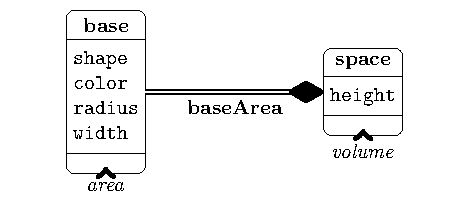
\includegraphics[width=1.2\textwidth]{../demonstrations/geometricShape/report/figures/factors}
\end{marginfigure}

The command \mcode{geometricShape('f')} generates a diagram view of the experiment.

\subsection{Process}

\begin{lstlisting}
geometricShape('do', 1);
\end{lstlisting}
run the base step over all 18 settings.
\begin{lstlisting}
geometricShape('do', 0, 'mask', {[1 2] 0 1});
\end{lstlisting}
runs successively every steps over the cylinders of radius 2  and all the pyramids.

\subsection{Expose observations}

Upon completion of the processing, the results of the last processing are displaying in the command window:

This display can be achieved by issuing the following command:
\begin{lstlisting}
geometricShape('display', 2, 'expose', '>', 'mask', {[1 2] 0 1});
\end{lstlisting}
The exposition of relevant observations is important for efficient computational experimentation. \expcode provides many tools for this purpose, type \mcode{help expExpose} for quick reference. 


The command:
\begin{lstlisting}
geometricShape('display', 2, 'mask', {1 0 1},...
 'expose', {'t', 'obs', 3, 'sort', 1});
\end{lstlisting}
\begin{marginfigure}
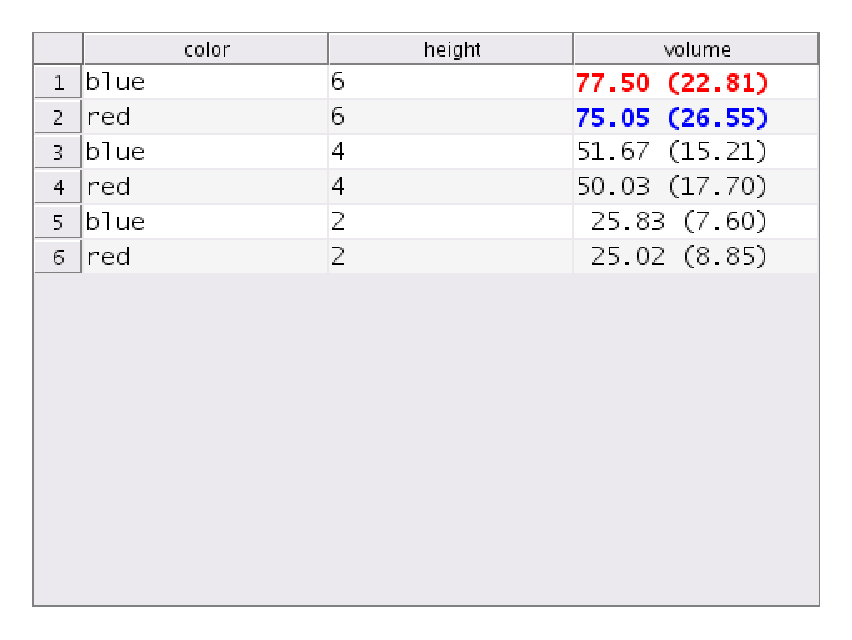
\includegraphics[trim={0 6cm 0 0},clip,width=1.2\textwidth]{../demonstrations/geometricShape/report/figures/mtable}
\end{marginfigure}
displays the volume (observation 3) of the step volume (2) for each cylinder of radius 2 sorted according to the first on a table (t). Red color indicates best performance, and blue ones, performances which are statistically equivalent to the best one. 
\marginnote{For this example, even if the blue cylinder is bigger than the blue one due to the uncertainty in the estimation of $\pi$, this difference is not significant, so the blue and red cylinders shall be considered of equivalent volume.}

\subsection{Report}

The file \mcode{<shortExperimentName>Report.m}, that is \mcode{geshReport.m} in this example allows you to generate report that compile several expositions of observations: Latex table (l), bar plot (b), and box plot (x).

\lstinputlisting[firstline=13, lastline=17]{../demonstrations/geometricShape/geshReport.m}

\input{../demonstrations/geometricShape/report/tables/geol}


\begin{marginfigure}
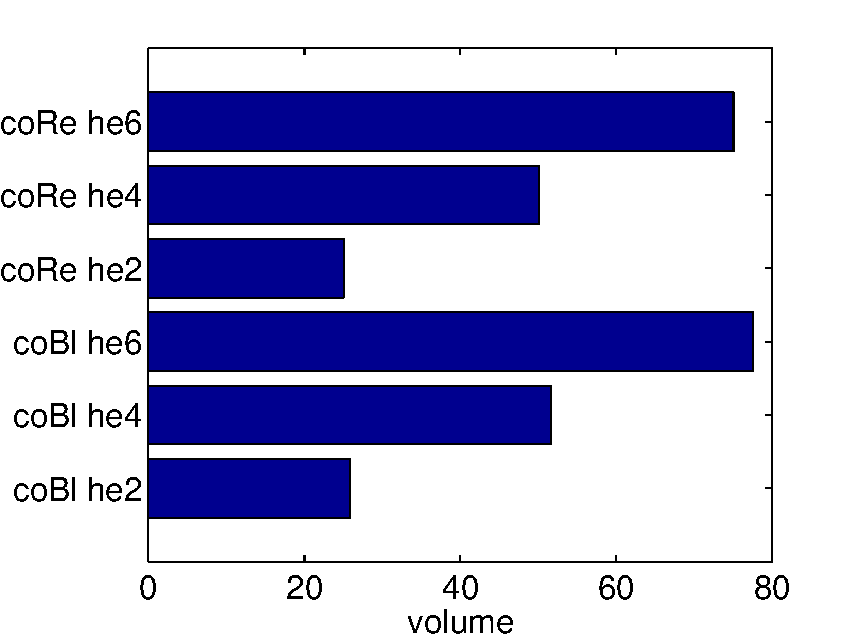
\includegraphics[clip,width=1.2\textwidth]{../demonstrations/geometricShape/report/figures/geob}
\end{marginfigure}



Several reports can be handled for the same experiment using the key \mcode{'reportName'}, and if the name of the report contain the key \mcode{'Slides'}, a slide presentation layout is used. For example, the command:
\begin{lstlisting}
geometricShape('report', 'rcv', ...
  'reportName', 'presentationSlides');
\end{lstlisting} 
generates a report with base name \mcode{presentationSlides} in a slides presentation layout.

\begin{marginfigure}
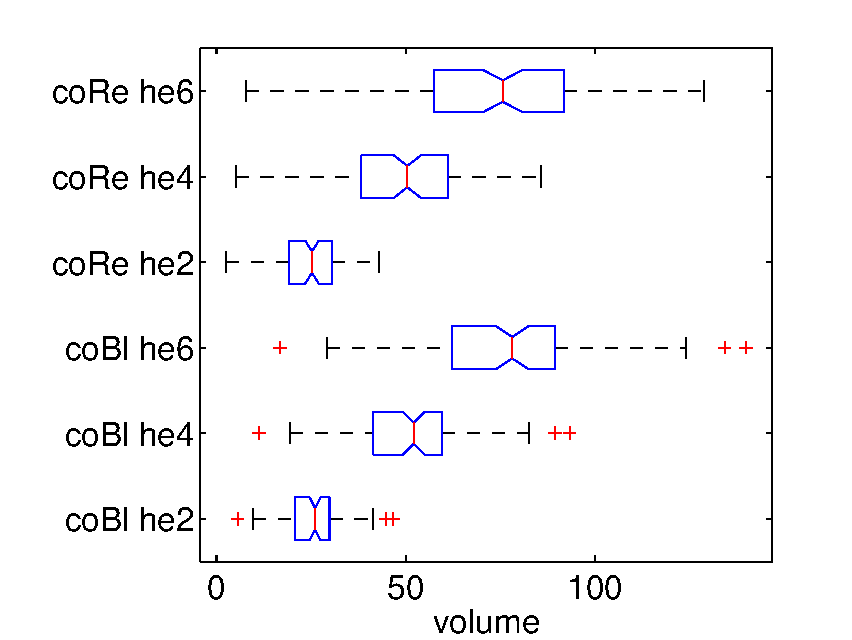
\includegraphics[clip,width=1.2\textwidth]{../demonstrations/geometricShape/report/figures/geox}
\end{marginfigure}

\section{Architecture of an experiment}

An \expcode experiment has a specific directory architecture. 

\subsection{Code}

The main directory hosts the main processing routines (named \mcode{codePath} in your configuration). It has the following files:
\begin{itemize}
\item \mcode{<projecName>}: main entry point of the experiment
\item \mcode{Factors}: text file encoding the factors of the experiment
\item \mcode{Init}: processed before any prcessing step
\item \mcode{Steps}: implement each processing units
\item \mcode{Report}: handle the generation of report that compile several types of expositions of observations
\end{itemize}

\subsection{Configuration}

The processing environment of the experiment can be controled with the files hosted in the directory \mcode{config}.

Almost every processing units of an \expcode experiment has access to a structure named \mcode{config} which is imported from a file which is specific to each user. This file is created at the creation of the experiment from a user specific file that can be found in the \mcode{.expCode} directory in the home directory of the user.

The syntax of this file allows the user to handle several configuration depending on which machine the experiment is processed. For example, let us assume that the project handles 3 machines with different file architectures:
\begin{lstlisting}
machineNames  = {{'toto', 'yoyo'}, 'dodo', 'momo'}
codePath = {'~/code/geometricShape', '/lab/code/geometricShape}
\end{lstlisting}
If the experiment is processed on the machine \mcode{'toto'}, or \mcode{'yoyo'}

Every entry of the configuration file can be overwritten at the command line call. For example:
\begin{lstlisting}
geometricShape('do', 0, 'sendMail', 1)
\end{lstlisting}
process every steps and sends an email at the end of the processing.

New entries can also be added and accessed in the processing files of the experiment:
\begin{lstlisting}
geometricShape('myEntry', 'toto')
\end{lstlisting}
outputs:
\begin{lstlisting}
Warning. The command line parameter myEntry is not found
 in the Config file. Setting anyway.
\end{lstlisting}


\subsection{Data}

Access to input data and processing data are respect


\subsection{Report}

\section{Commands}

\subsection{Management of an experiment}

\subsection{Computation of settings}

\subsection{Exposition of observations}

\section{Best practices} \label{sec:best}

factorial design

multi way anova

\section{Recommended readings}

\begin{itemize}


\item \textbf{Getting it right}: R\&D Methods for Science and Engineering, Peter Bock, Academic Press

\item \textbf{The Visual Display of Quantitative Information} Edward R. Tufte

\end{itemize}







main concepts

experiment statement

factors, modalities

processing

processing steps

parallelization, independance, sequentiality

factorial tree

data / observations

Main steps

definition
computation
mining
reporting

distant computing
data retrieval

\bibliographystyle{plain}
\bibliography{references}

\end{document}